\textbf{The Effects of Training Hyperparameters.} To deepen our analysis, we further conduct experiments that vary core training hyperparameters—specifically, the number of continual pre-training (CPT) epochs and the learning rate—and analyze their impact on model performance.
By default, we use \llama. 

Table \ref{tab:epoch-merged} presents the effects of the \textbf{number of epochs} on the ARC and Ruler benchmarks. We have two major observations: (1) Just after one epoch of CPT, models trained on higher junk-data ratios already show clear declines in performance, indicating that the negative effects are not simply due to catastrophic forgetting or overfitting. The \emph{early occurrence} of Brain Rot effects indicates that the decline originates from the intrinsic deficiencies of junk data itself, which negatively affects model reasoning and generalization even under minimal CPT exposure. (2) Additional epochs amplify the observed degradation, but the underlying pattern remains consistent. Regardless of training duration, models trained on cleaner control data consistently outperform those exposed to 'junk' data.


% \begin{table}[h]
% \centering
% \footnotesize
% \setlength{\tabcolsep}{6pt}
% \caption{Performance of Llama-8B-Instruct under varying junk-data ratios across one and two epochs of continual pre-training.}
% \label{tab:epoch-merged}
% \begin{tabular}{lccccc|ccccc}
% \toprule
% & \multicolumn{5}{c}{\textbf{One Epoch}} 
% & \multicolumn{5}{c}{\textbf{Two Epochs}} \\
% \cmidrule(lr){2-6} \cmidrule(lr){7-11}
% \textbf{Task} 
% & 100\% & 80\% & 50\% & 20\% & 0\% 
% & 100\% & 80\% & 50\% & 20\% & 0\% \\
% \midrule
% ARC\_Easy 
% & 74.11 & 75.33 & 76.76 & 77.27 & 78.91
% & 73.44 & 74.41 & 74.78 & 76.09 & 78.87 \\
% ARC\_Challenge 
% & 42.23 & 43.51 & 46.58 & 48.03 & 48.72
% & 44.28 & 44.28 & 43.94 & 46.41 & 48.97 \\
% Ruler 
% & 90.88 & 90.31 & 90.10 & 91.38 & 91.28
% & 89.19 & 89.08 & 90.30 & 92.11 & 90.92 \\
% \bottomrule
% \end{tabular}
% \end{table}

% \begin{table}[h]
% \centering
% \footnotesize
% \setlength{\tabcolsep}{6pt}
% \caption{Performance of Llama-8B-Instruct under varying junk-data ratios across one and two epochs of continual pre-training.}
% \label{tab:epoch-merged}
% \begin{tabular}{lccccc|ccccc}
% \toprule
% & \multicolumn{5}{c}{\textbf{One Epoch}} 
% & \multicolumn{5}{c}{\textbf{Two Epochs}} \\
% \cmidrule(lr){2-6} \cmidrule(lr){7-11}
% \textbf{Task} 
% & 100\% & 80\% & 50\% & 20\% & 0\% 
% & 100\% & 80\% & 50\% & 20\% & 0\% \\
% \midrule
% ARC Easy 
% & 73.21 & 74.12 & 76.81 & 77.49 & 77.92
% & 72.67 & 73.01 & 75.14 & 75.39 & 76.04 \\
% ARC Challenge 
% & 43.76 & 43.88 & 45.19 & 47.51 & 47.10
% & 43.92 & 44.02 & 43.72 & 46.75 & 46.51 \\
% Ruler 
% & 72.34 & 83.21 & 83.13 & 91.13 & 91.71
% & 71.41 & 81.69 & 81.10 & 90.74 & 89.97 \\
% \bottomrule
% \end{tabular}
% \end{table}

\begin{table}[h]
\centering
\footnotesize
\setlength{\tabcolsep}{2pt}
\caption{Performance of Llama-8B-Instruct under varying junk-data ratios across one and two epochs of continual pre-training.}
\label{tab:epoch-merged}
\begin{tabular}{lccc|ccc|ccc}
\toprule
\textbf{Junk Ratio}
& \multicolumn{3}{c|}{\textbf{One Epoch}}
& \multicolumn{3}{c}{\textbf{Two Epochs}} 
& \multicolumn{3}{c}{\textbf{Three Epochs}} \\
\cmidrule(lr){2-4}\cmidrule(lr){5-7}\cmidrule(lr){8-10}
& \textbf{ARC Easy} & \textbf{ARC Challenge} & \textbf{Ruler}
& \textbf{ARC Easy} & \textbf{ARC Challenge} & \textbf{Ruler}
& \textbf{ARC Easy} & \textbf{ARC Challenge} & \textbf{Ruler} \\
\midrule
100\% & 73.21 & 43.76 & 72.34 
& 72.67 & 43.92 & 71.41 
& 70.2 & 41.6 & 71.0\\
80\%  & 74.12 & 43.88 & 83.21 
& 73.01 & 44.02 & 81.69 
& 71.7 & 44.5 & 79.0\\
50\%  & 76.81 & 45.19 & 83.13 
& 75.14 & 43.72 & 81.10 
& 74.2 & 43.4 & 80.0\\
20\%  & 77.49 & 47.51 & 91.13 
& 75.39 & 46.75 & 90.74 
& 75.5 & 46.2 & 89.7\\
0\%   & 77.92 & 47.10 & 91.71 
& 76.04 & 46.51 & 89.97 
& 75.6 & 46.2 & 89.7\\
\bottomrule
\end{tabular}
\end{table}



In Table \ref{tab:lr-results}, we report the model performance by varying the \textbf{learning rate} during CPT. 
(1)~Using a larger learning rate ($1\times10^{-4}$) significantly exacerbates the degradation and accelerates the ``Brain Rot'', allowing the low-quality data to rapidly overwrite the model's pre-trained knowledge.
(2)~Smaller learning rates ($1\times10^{-6}$) essentially mitigate this decline. By dampening the magnitude of the updates, the model restricts the extent of representational drift, thereby retaining more of its original capabilities despite exposure to the junk distribution.
However, along with mitigation, smaller learning also causes poorer training effects: the CPT loss decreases from $4.57$ to only $3.03$ (learning rate of $1\times10^{-6}$), which is much higher than $2.20$ by learning rate of $1\times10^{-4}$.

% \begin{table}[h]
% \centering
% \footnotesize
% \setlength{\tabcolsep}{6pt}
% \caption{Performance under different junk-data ratios for continual pre-training at learning rates $1\times10^{-4}$ and $1\times10^{-6}$.}
% \label{tab:lr-results}
% \begin{tabular}{lccccc|ccccc}
% \toprule
% & \multicolumn{5}{c}{\textbf{Learning Rate: $1\times10^{-4}$}} 
% & \multicolumn{5}{c}{\textbf{Learning Rate: $1\times10^{-6}$}} \\
% \cmidrule(lr){2-6} \cmidrule(lr){7-11}
% \textbf{Task} 
% & 100\% & 80\% & 50\% & 20\% & 0\%
% & 100\% & 80\% & 50\% & 20\% & 0\% \\
% \midrule
% ARC\_Easy 
% & 40.53 & 43.69 & 52.15 & 60.10 & 68.22
% & 76.73 & 76.89 & 77.23 & 77.82 & 78.66 \\
% ARC\_Challenge 
% & 24.23 & 25.94 & 30.03 & 35.75 & 38.48
% & 47.53 & 48.46 & 48.29 & 49.74 & 50.09 \\
% Ruler
% & 7.84 & 4.68 & 10.22 & 23.59 & 45.67
% & 94.42 & 94.16 & 94.53 & 94.39 & 94.58 \\
% \bottomrule
% \end{tabular}
% \end{table}



% \begin{table}[h]
% \centering
% \footnotesize
% \setlength{\tabcolsep}{6pt}
% \caption{Performance under different junk-data ratios for continual pre-training at learning rates $1\times10^{-4}$ and $1\times10^{-6}$.}
% \label{tab:lr-results}
% \begin{tabular}{lccccc|ccccc}
% \toprule
% & \multicolumn{5}{c}{\textbf{Learning Rate: $1\times10^{-4}$}} 
% & \multicolumn{5}{c}{\textbf{Learning Rate: $1\times10^{-6}$}} \\
% \cmidrule(lr){2-6} \cmidrule(lr){7-11}
% \textbf{Task} 
% & 100\% & 80\% & 50\% & 20\% & 0\%
% & 100\% & 80\% & 50\% & 20\% & 0\% \\
% \midrule
% ARC Easy 
% & 42.54 & 47.16 & 54.92 & 63.01 & 68.21
% & 77.19 & 77.40 & 78.43 & 78.81 & 79.25 \\
% ARC Challenge 
% & 25.17 & 25.91 & 31.07 & 34.58 & 37.04
% & 46.33 & 47.07 & 48.50 & 48.91 & 50.37 \\
% Ruler
% & 11.62 & 10.49 & 13.96 & 26.89 & 40.31
% & 87.63 & 89.74 & 90.62 & 91.13 & 91.90 \\
% \bottomrule
% \end{tabular}
% \end{table}

\begin{table}[h]
\centering
\footnotesize
\setlength{\tabcolsep}{2pt}
\caption{Performance under different junk-data ratios for continual pre-training at different learning rates.}
\label{tab:lr-results}
\begin{tabular}{c|ccc|ccc|ccc}
\toprule
\textbf{Junk Ratio} 
& \multicolumn{3}{c|}{\textbf{Learning Rate: $1\times10^{-4}$}}
& \multicolumn{3}{c|}{\textbf{Learning Rate: $1\times10^{-5}$}}
& \multicolumn{3}{c}{\textbf{Learning Rate: $1\times10^{-6}$}} \\
\cmidrule(lr){2-4}\cmidrule(lr){5-7}\cmidrule(lr){8-10}
& \textbf{ARC Easy} & \textbf{ARC Challenge} & \textbf{Ruler}
& \textbf{ARC Easy} & \textbf{ARC Challenge} & \textbf{Ruler}
& \textbf{ARC Easy} & \textbf{ARC Challenge} & \textbf{Ruler} \\
\midrule
100\% & 42.5 & 25.2 & 11.6
& 70.2 & 41.6 & 71.0
& 77.2 & 46.3 & 87.6 \\
80\%  & 47.2 & 25.9 & 10.5 
& 71.7 & 44.5 & 79.0
& 77.4 & 47.1 & 89.7 \\
50\%  & 54.9 & 31.1 & 13.9
& 74.2 & 43.4 & 80.0
& 78.4 & 48.5 & 90.6 \\
20\%  & 63.0 & 34.6 & 26.9 
& 75.5 & 46.2 & 89.7
& 78.8 & 48.9 & 91.1 \\
0\%   & 68.2 & 37.0 & 40.3 
& 75.6 & 46.2 & 89.7
& 79.3 & 50.4 & 91.9 \\
\bottomrule
\end{tabular}
\end{table}


\textbf{The Effects of Model Scale.} To further examine the role of model scale, we conduct an additional experiment using Llama3-70B-Instruct~\citep{llama3} as the backbone, following the same setup described in Section \ref{sec:control-exp}. 
% Due to limited academic computing resources, we were only able to complete training on the 100\% junk data (M1) and evaluation on the ARC benchmark. 
The results are summarized in Table \ref{tab:arc_junk_70b}.
We observe that, despite the significantly larger parameter size, the effect of brain rot on reasoning still clearly persists, especially in complex reasoning tasks (ARC-Challenge dropped by over 5 percent). This is consistent with the trend observed in smaller models, indicating that increased model size alone does not effectively mitigate the impact of junk-data exposure.

\begin{table}[ht]
\centering
\small
\caption{Performance under 100\% Junk (M1) with Llama3-70B-Instruct as the backbone.}
\setlength{\tabcolsep}{6pt}
\begin{tabular}{lccc}
\toprule
\textbf{Task} & \textbf{Base} & \textbf{100\% Junk (M1)} & \textbf{$\Delta$} \\
\midrule
ARC Easy      & 82.4 & 80.1 & -2.3 \\
ARC Challenge & 57.8 & 52.7 & -5.0 \\
\bottomrule
\end{tabular}
\label{tab:arc_junk_70b}
\end{table}


\textbf{Continual Control Training.} 
Following the same setup as the post-hoc tuning in Section \ref{sec:mitigation}, we further perform continual control training (CCT) to mitigate the effects of the junk intervention, using control data scaled from 0 to 1.2 million tokens (the maximum). Each CCT run is subsequently followed by instruction tuning. As shown in Figure \ref{fig:wash-out_scaling-control}, CCT demonstrate a scaling trend similar to that of CPT, and both are less effective than IT. This indicates that the effects introduced by junk intervention are difficult to mitigate through post-hoc continual training on control data.

\begin{figure}[ht]
    \centering
    % \textbf{(c)}\\[-2pt]
    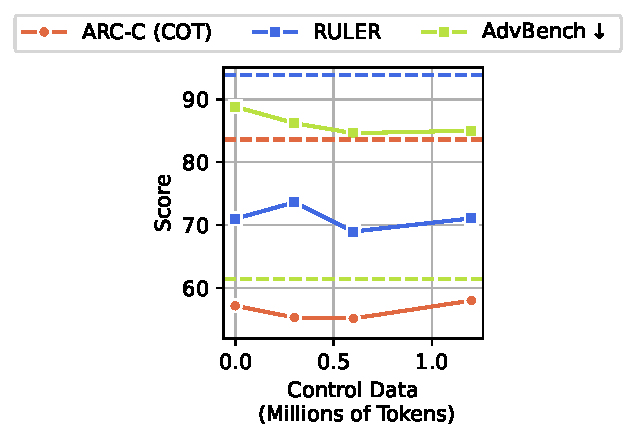
\includegraphics[width=0.45\linewidth]{figs/wash_out_scaling_control_only.pdf}
    \caption{Scaling post-hoc continual control training (CCT). Dashed lines indicate the baseline models.}
    \label{fig:wash-out_scaling-control}
\end{figure}